\documentclass[12pt]{article}
\usepackage[utf8]{inputenc}
\usepackage{hyperref}
\usepackage{graphicx}
\usepackage{float}
\usepackage{xcolor}
%Insert tab
\providecommand{\tab}{\hspace{10pt}}
\bibliographystyle{ieeetr}
\title{SPIFI Improvements Report}
\author{Brennan W. Fieck}
\begin{document}
\begin{titlepage}
\clearpage\maketitle
\thispagestyle{empty}
\begin{figure}[H]
\centering

\includegraphics[width=0.5\textwidth]{team-logo.png}
\end{figure}
\end{titlepage}

\section*{Introduction}
The basis of the broader project to which this team's efforts contribute
is to expand upon an existing technology called  Spatial Frequency
Modulated Single Detector Imaging (SPIFI). This team created simulation
software and measurement software dealing with potential improvements to
the SPIFI technique. The simulation served as a proof-of-concept as well
as a helpful guide for what has come to be known as "2D-SPIFI". The measurement software is used to implement photon-counting rather than conventional detection methods.

\section*{Background}
SPIFI is a revolutionary imaging technique that allows a line to be scanned
across an object by a single laser at one time, without using a raster pattern
along the line. This represents a performance change from $O[n^2]$ to $O[n]$ for a square object with side length $n$. SPIFI accomplishes this by encoding the information about an object in a
frequency change which maps directly to a spatial line that spans the object,
and which evolves in time as the line sweeps over the object. Traditionally, scanning more than a single point at a time
would require multiple collectors to be able to
resolve which photons were used to scan what part of the object (e.g.
using a camera). Figure \ref{fig:cube-line} depicts part of a very simple SPIFI system being used to image a gray cube.

\begin{figure}[ht]
	\centering
	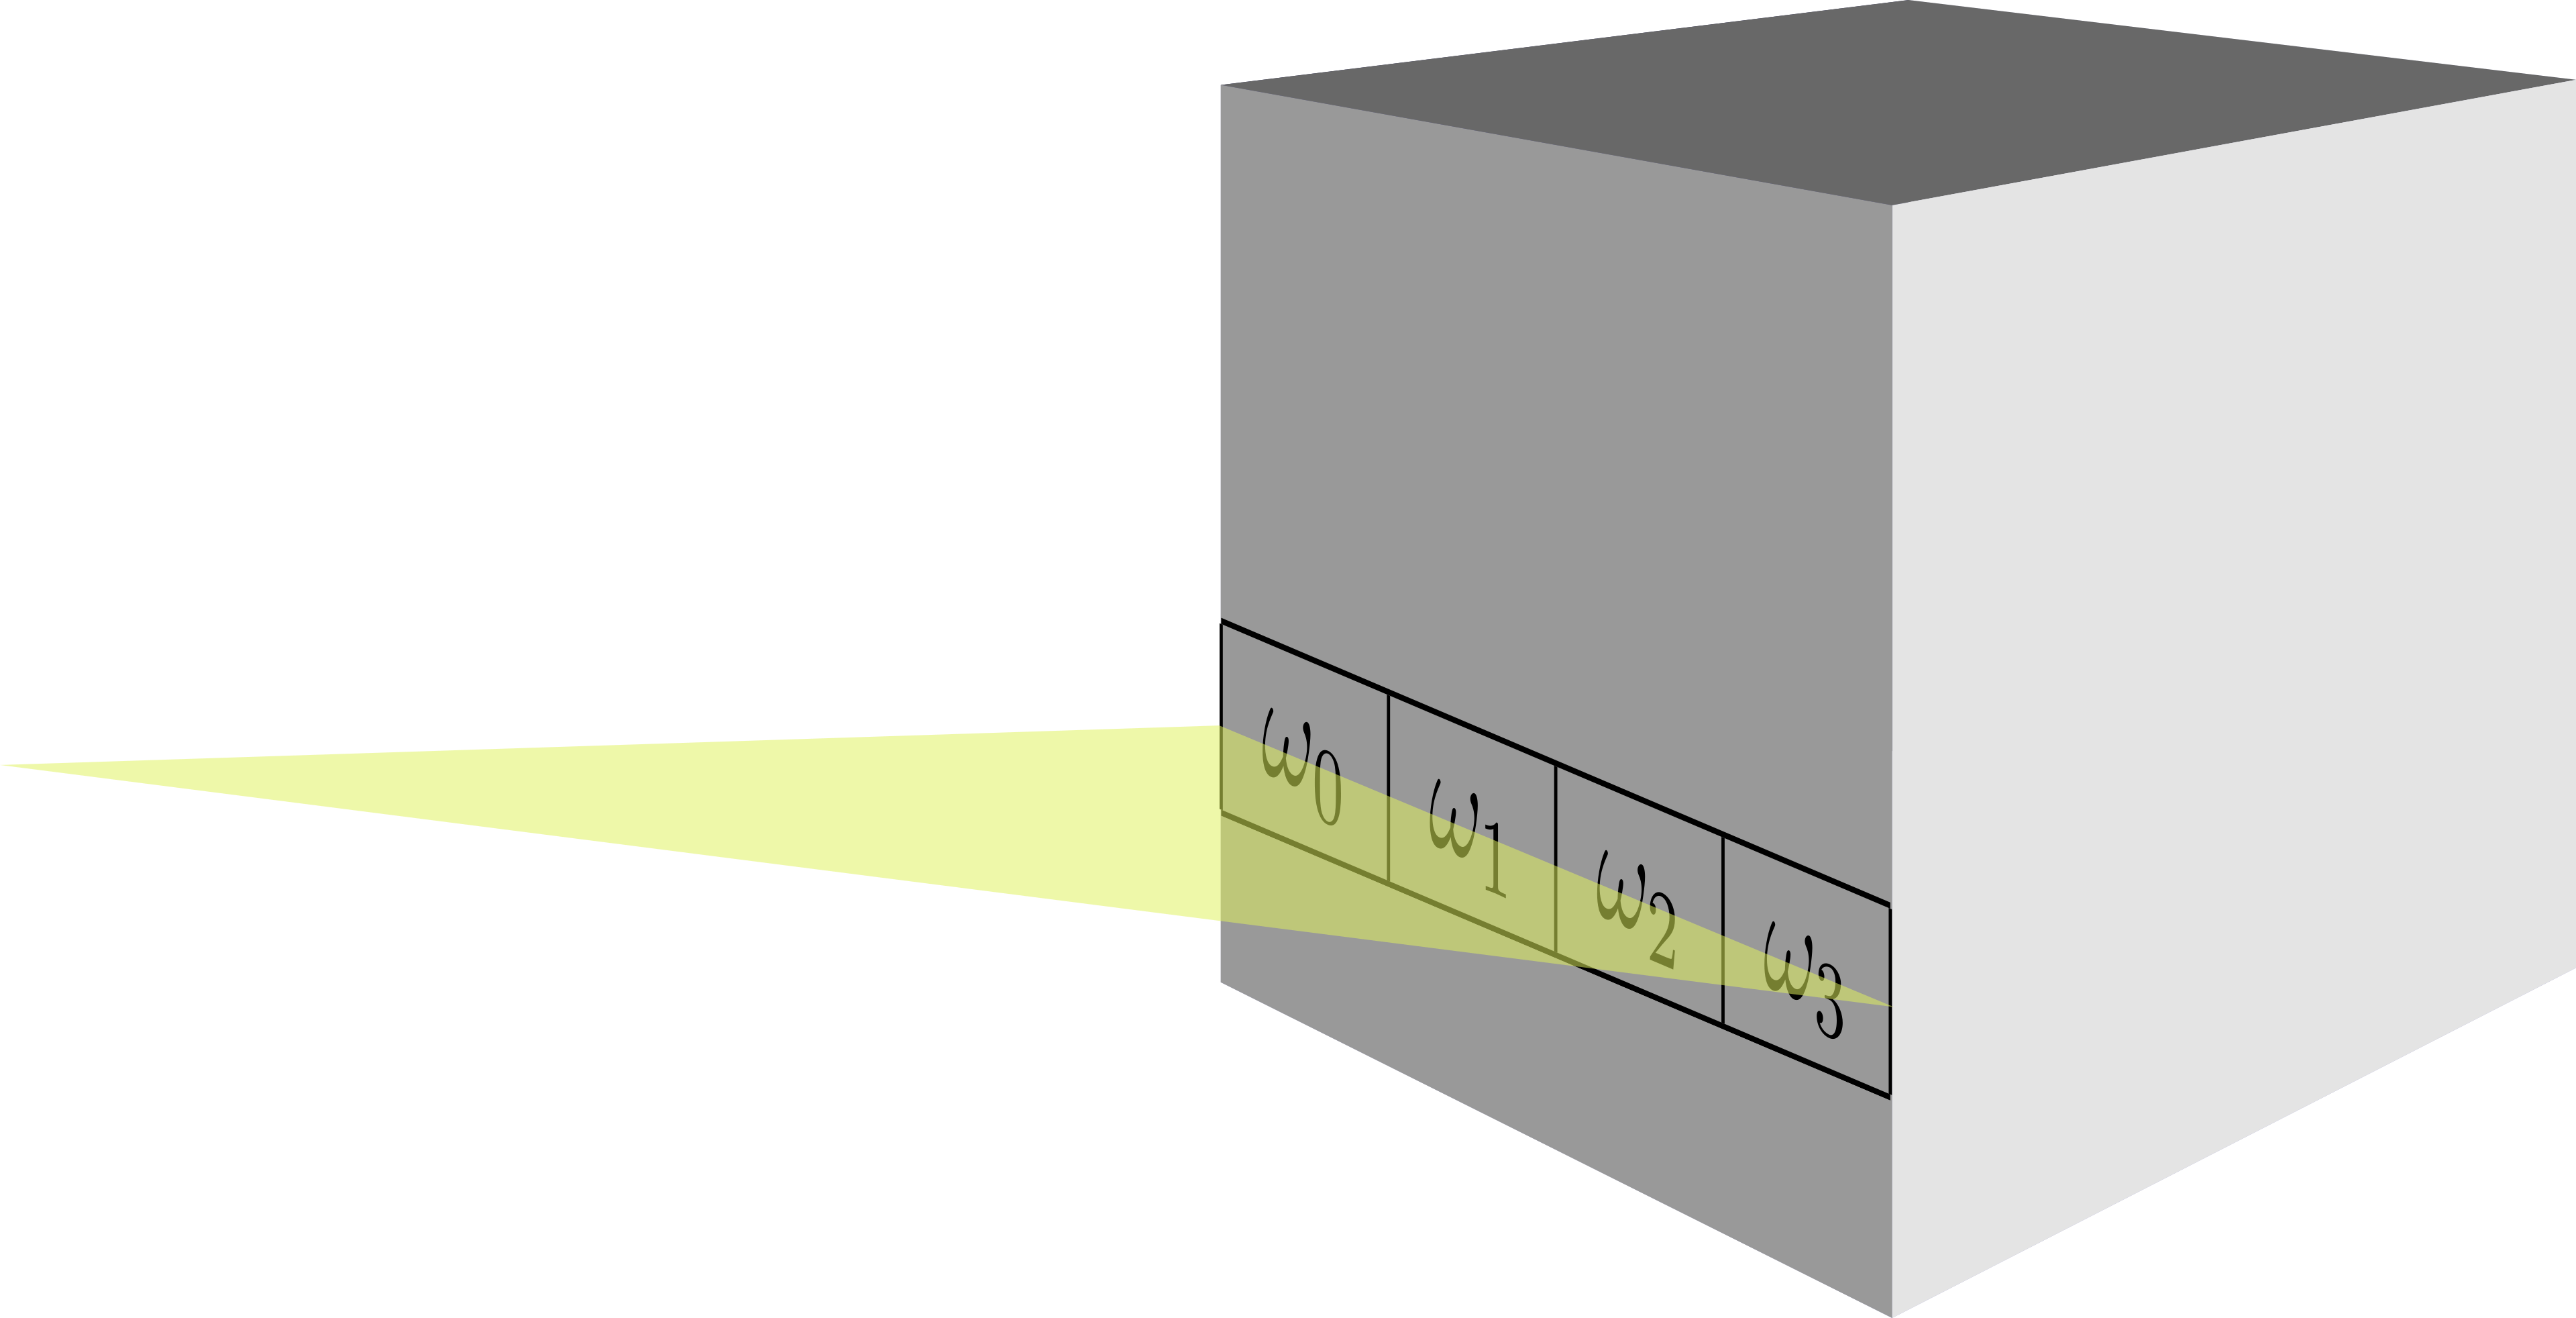
\includegraphics[width=0.75\textwidth]{spifi-line-on-cube.png}
	\caption{Visual Depiction of Spatial Frequency Mapping}
	\label{fig:cube-line}
\end{figure}

The four $\omega$s in boxes represent different, unique frequencies along the plane of light hitting the object. Of course, in practice the frequency modulation is smoother and the resolution of the imaging is determined by how many "boxes" one can make on the face of the object. The sheet of light is mechanically swept across the object, and as it moves the frequencies each evolve in a consistently unique manner. Figure \ref{fig:cube-sheet} shows how frequency varies in time as the sheet of light sweeps over the object.

\begin{figure}[ht]
	\centering
	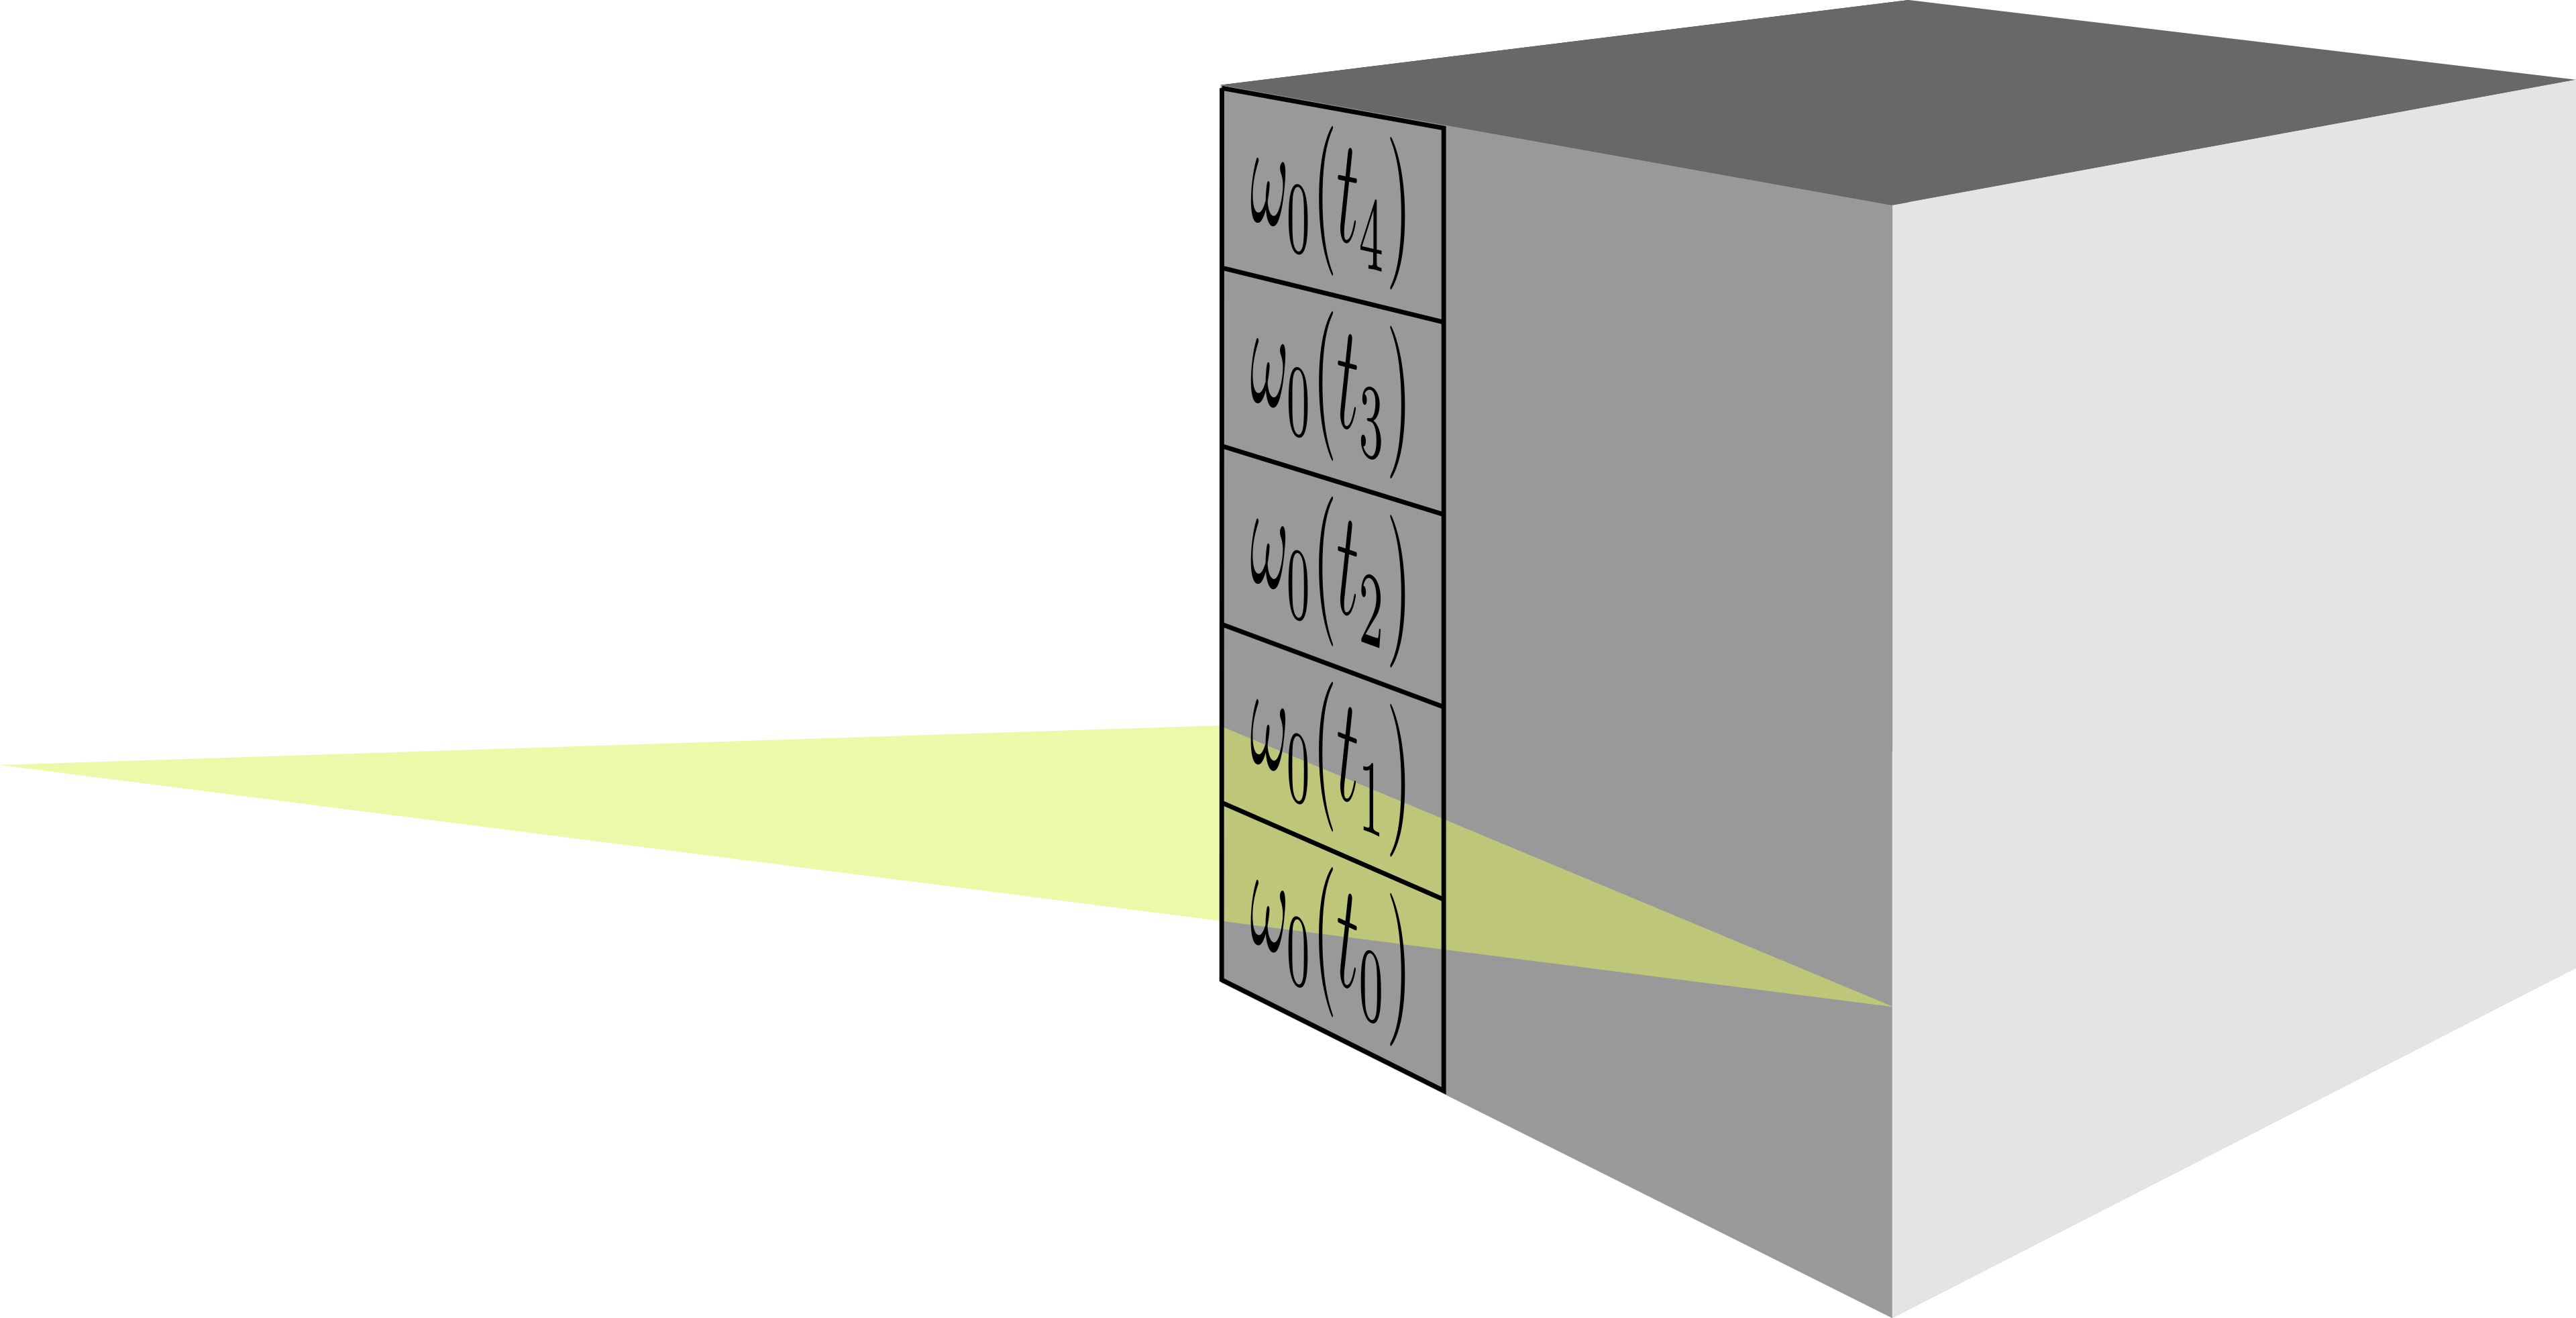
\includegraphics[width=0.75\textwidth]{spifi-sheet-on-cube}
	\caption{Visual Depiction of Temporal Frequency Mapping}
	\label{fig:cube-sheet}
\end{figure}



\begin{figure}[ht]
\centering
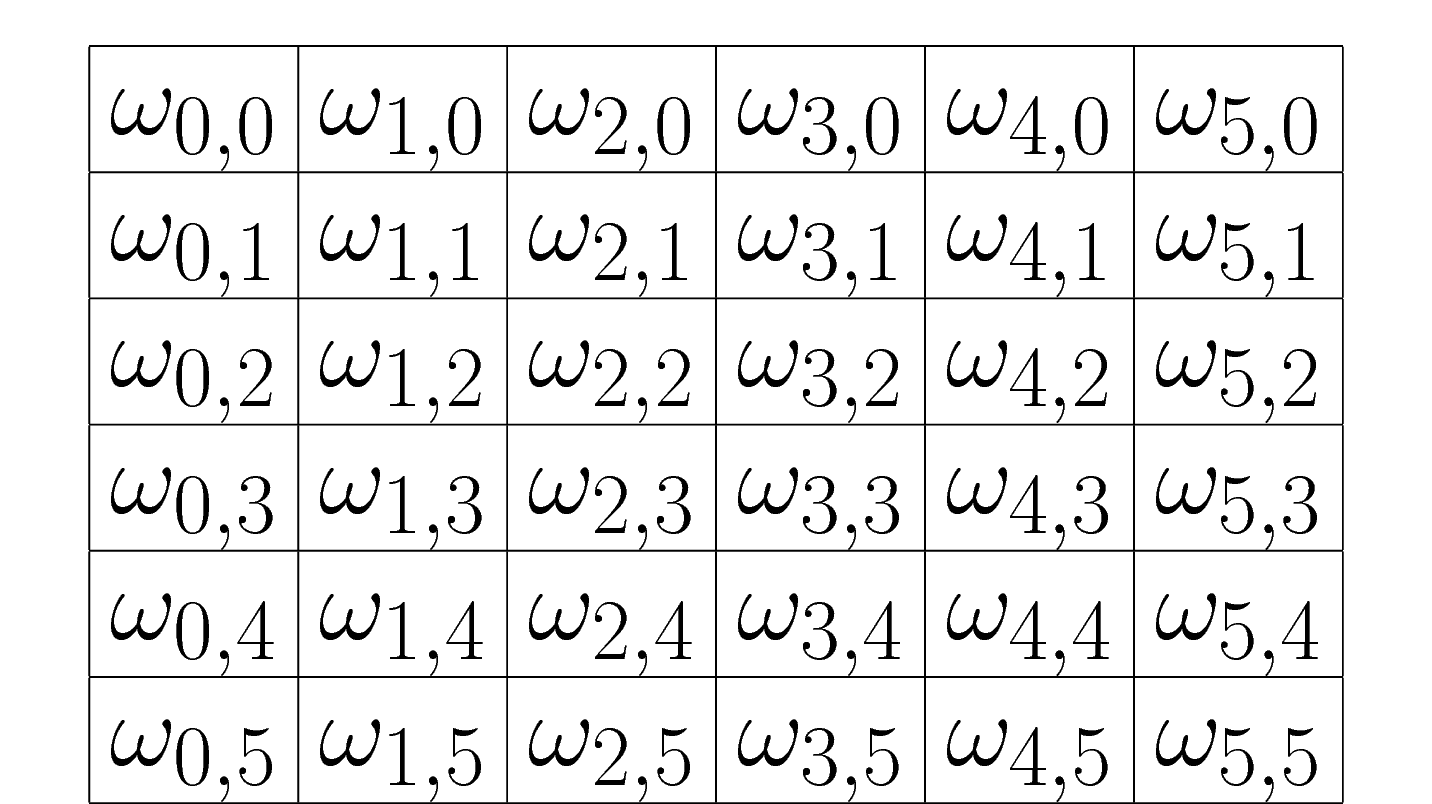
\includegraphics[width=0.75\textwidth]{spifi-grid.png}
\caption{Total Frequency Mapping Over an Object\label{fig:mapping-diagram}}
\end{figure}

Figure \ref{fig:mapping-diagram} shows the net result of these temporal and spacial frequency mappings;
each inscribed $\omega$ is unique to the section of the
$x/y$ plane that bounds it. After passing through the object, the light is gathered back into a well-collimated beam and collected by a single-pixel detector. Then decomposing the measured signal into the frequencies that make it up allows for inspection of how the laser interacted with the object at specific points on its surface. Each of these tiny "boxes" as seen in Figure \ref{fig:mapping-diagram} can be interpreted directly as a pixel. This is done by measuring the attenuation of the specific frequency. For example, considering once again Figure \ref{fig:mapping-diagram}, suppose that the measured signal has almost none of the frequency $\omega_{2,2}$ in it, but has nearly all of the $\omega_{0,0}$ that it started with. This means that light in the upper-left corner of the object faced almost no resistance, while nearly all of that which traveled through $(x,y)=(2,2)$ was blocked. It's then reasonable to conclude that the object is shaped such that it is relatively thick at $(2,2)$, and relatively thin at $(0,0)$.

% \begin{figure}[ht]
% \centering
% 
\includegraphics[width=0.75\textwidth]{spifi-system}
% \caption{A Simple SPIFI System Setup\label{fig:spifi-sys}}
% \end{figure}

\begin{figure}[ht]
\centering
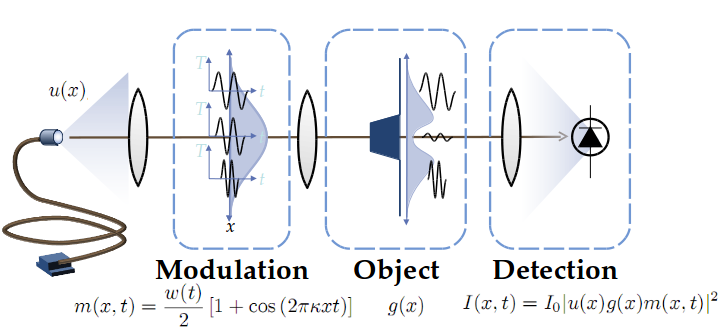
\includegraphics[width=0.75\textwidth]{spifi-system-graphical}
\caption{A Simple SPIFI System\label{fig:spifi-sys}}
\end{figure}

This frequency mapping is achieved by spreading the laser into a sheet and then passing it through a SPIFI mask. Designs of these masks vary, but they can all be understood in the same manner through their transfer function acting on the laser. Figure
\ref{fig:spifi-sys} shows the signal transfer system, starting with some laser given by $u(x)$. The modulation function shown, $m(x,t)$, is then applied, followed by the laser passing through the object which itself applies some unkown transfer function $g(x)$. The final result measured on the detector is an intensity, so only the square of the signal is observable.
The transfer function $g[x,y]$ is determined
by the object being
imaged, and represents an attenuation of amplitude of specific sections of the
$xy$ plane based on the object's ability to absorb and reflect light.
Typically this function is used to describe the object, and once found will immediately yield an image of the object.

\begin{figure}[H]

\includegraphics[width=0.4\textwidth]{spinner}
\hfill

\includegraphics[width=0.4\textwidth]{rectangular_spifi_mask}
\caption{Left: A Circular SPIFI Mask -
Right: A Rectangular SPIFI Mask\label{fig:ex-grat}}
\end{figure}

Examples of typical SPIFI masks are
shown in Figure \ref{fig:ex-grat}. For the common circular mask - 
similar to the one in the figure - the form of the pattern in polar
coordinates is
\begin{equation}
\textnormal{pattern}[r,t]=\frac{1}{2}+\frac{1}{2}\cos\left[2\pi
f_mk_prt\right].
\label{eq:pattern}
\end{equation}

Here, $f_m$ is the rotational of the mask, and $k_p$ is a constant
that has to do with the density of the lines in the pattern.

\begin{figure}[H]
\centering
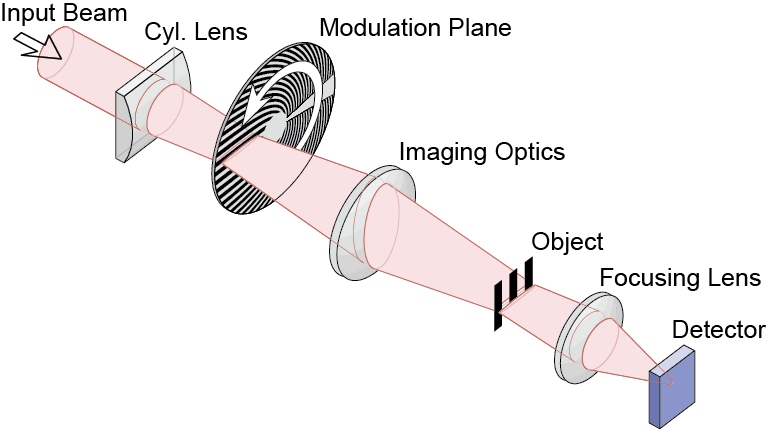
\includegraphics[width=0.75\textwidth]{circular_SPIFI_system}
\caption{A Simple SPIFI System Using a Circular Mask}
\label{fig:circ-sys}
\end{figure}

As shown in Figure \ref{fig:circ-sys}, this function modulates the laser as it passes
through the mask as a line, and then is scanned along the object from top
to bottom by a mechanical apparatus twisting a lens or mirror. A transformation from Equation
\ref{eq:pattern} to the $m[x,y,t]$ transfer function requires sampling the
output in intervals of $\tau_m=1/f_m$, the period of the pattern's 
spinning. 

Once the light has been scanned over the object, the intensity recorded by
the detector during $\tau_m$ can be Fourier-transformed to find the
contributions from each frequency at a given time. The time-domain and frequency-domain plots of this for some
unknown object looks like Figure \ref{fig:fourier}. 

\begin{figure}[H]
\centering
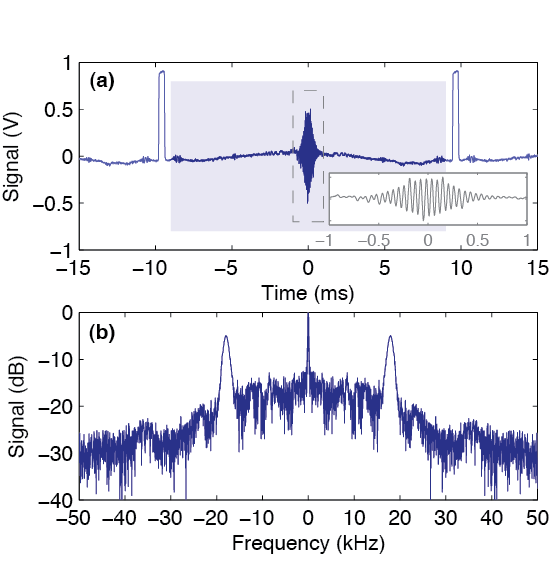
\includegraphics[width=0.75\textwidth]{Fourier_Transform}
\caption{Top: Time-Domain SPIFI Output - Bottom: Corresponding Frequency-Domain SPIFI Output\label{fig:fourier}}
\end{figure}

\section*{Theory of 2D SPIFI}
One focus of this project was to expand the capabilities of SPIFI by using a
mask which modulates the entire beam in two dimensions at any one time,
thereby eliminating the need to mechanically scan the laser along the object. 2D-SPIFI can scan an object in constant, or $O[1]$ time, as opposed to the current technique which has a complexity of $O[n]$ where $n$ is the size of the object - and again all of this is compared to $O[n^2]$ when using traditional raster-scan techniques. This technology is still in its infancy, but if it proves reliable wil obviously vastly improve real-time imaging. As a proof-of-concept, as well as to aid in the design of 2D SPIFI masks, the team produced software capable of simulating 2D-SPIFI for more or less arbitrary objects and masks.

\begin{figure}[ht]
	\centering
	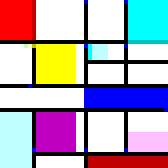
\includegraphics[width=0.45\textwidth]{testimg}
	\hfill
	
\includegraphics[width=0.45\textwidth]{testoutput}
	\caption{Left: Simulation Input "Object" - Right: Simulation Output Image}
	\label{fig:sim-in-out}
\end{figure}

Figure \ref{fig:sim-in-out} shows the input and output of the simulation when run using an image file as a representation of the object.

\section*{Photon Counting}
Previously, SPIFI measurements were taken using National Instruments$^\textnormal{\small TM}$ (NI) devices and passed through NI's proprietary LabView software for analysis. With the improved scanning speed expected from implementations of 2D-SPIFI, it will be necessary to increase processing of collected data as well. If one were able to count the photons incident on the detector, it would eliminate the need to perform Fourier transforms on the input. The energy of the photon will show up in the detection method  and therefore automatically carry the information about its frequency; e.g. photo-multiplier tubes produce current proportional to detected photon energy. So the mapping information is there and the image can begin being constructed immediately, each detected photon can be immediately added to a real-time image without the need for further computation. As a first step, attempts were made to connect a GPIB device - already owned by the lab and capable counting photons - to a desktop computer. However, it was determined that too much time would be spent getting the usb CPIB board to interface properly with a modern computer which could otherwise be spent on a more stable framework. The computation is simple enough to be carried out efficiently by a micro-controller, so a program was devised by the teamfor a Field-Programmable Gate Array (FPGA) as a first step in moving towards a headless data store. The design is fairly simple, it works by taking only two signals as inputs on the general-purpose I/O pins on the DEO-Nano FPGA. One is a reading of the laser control itself, which tells the FPGA when the laser fires a burst of photons, so that it can count them for that time period. The other input comes from the photo-multiplier tube that served as the detector. Then all the FPGA does is print a list of photons it counts during each laser pulse back through a usb cable to a normal computer. Figure \ref{fig:timing} shows an example of these signals, with the counting periods indicated.

\begin{figure}[ht]
	\centering
	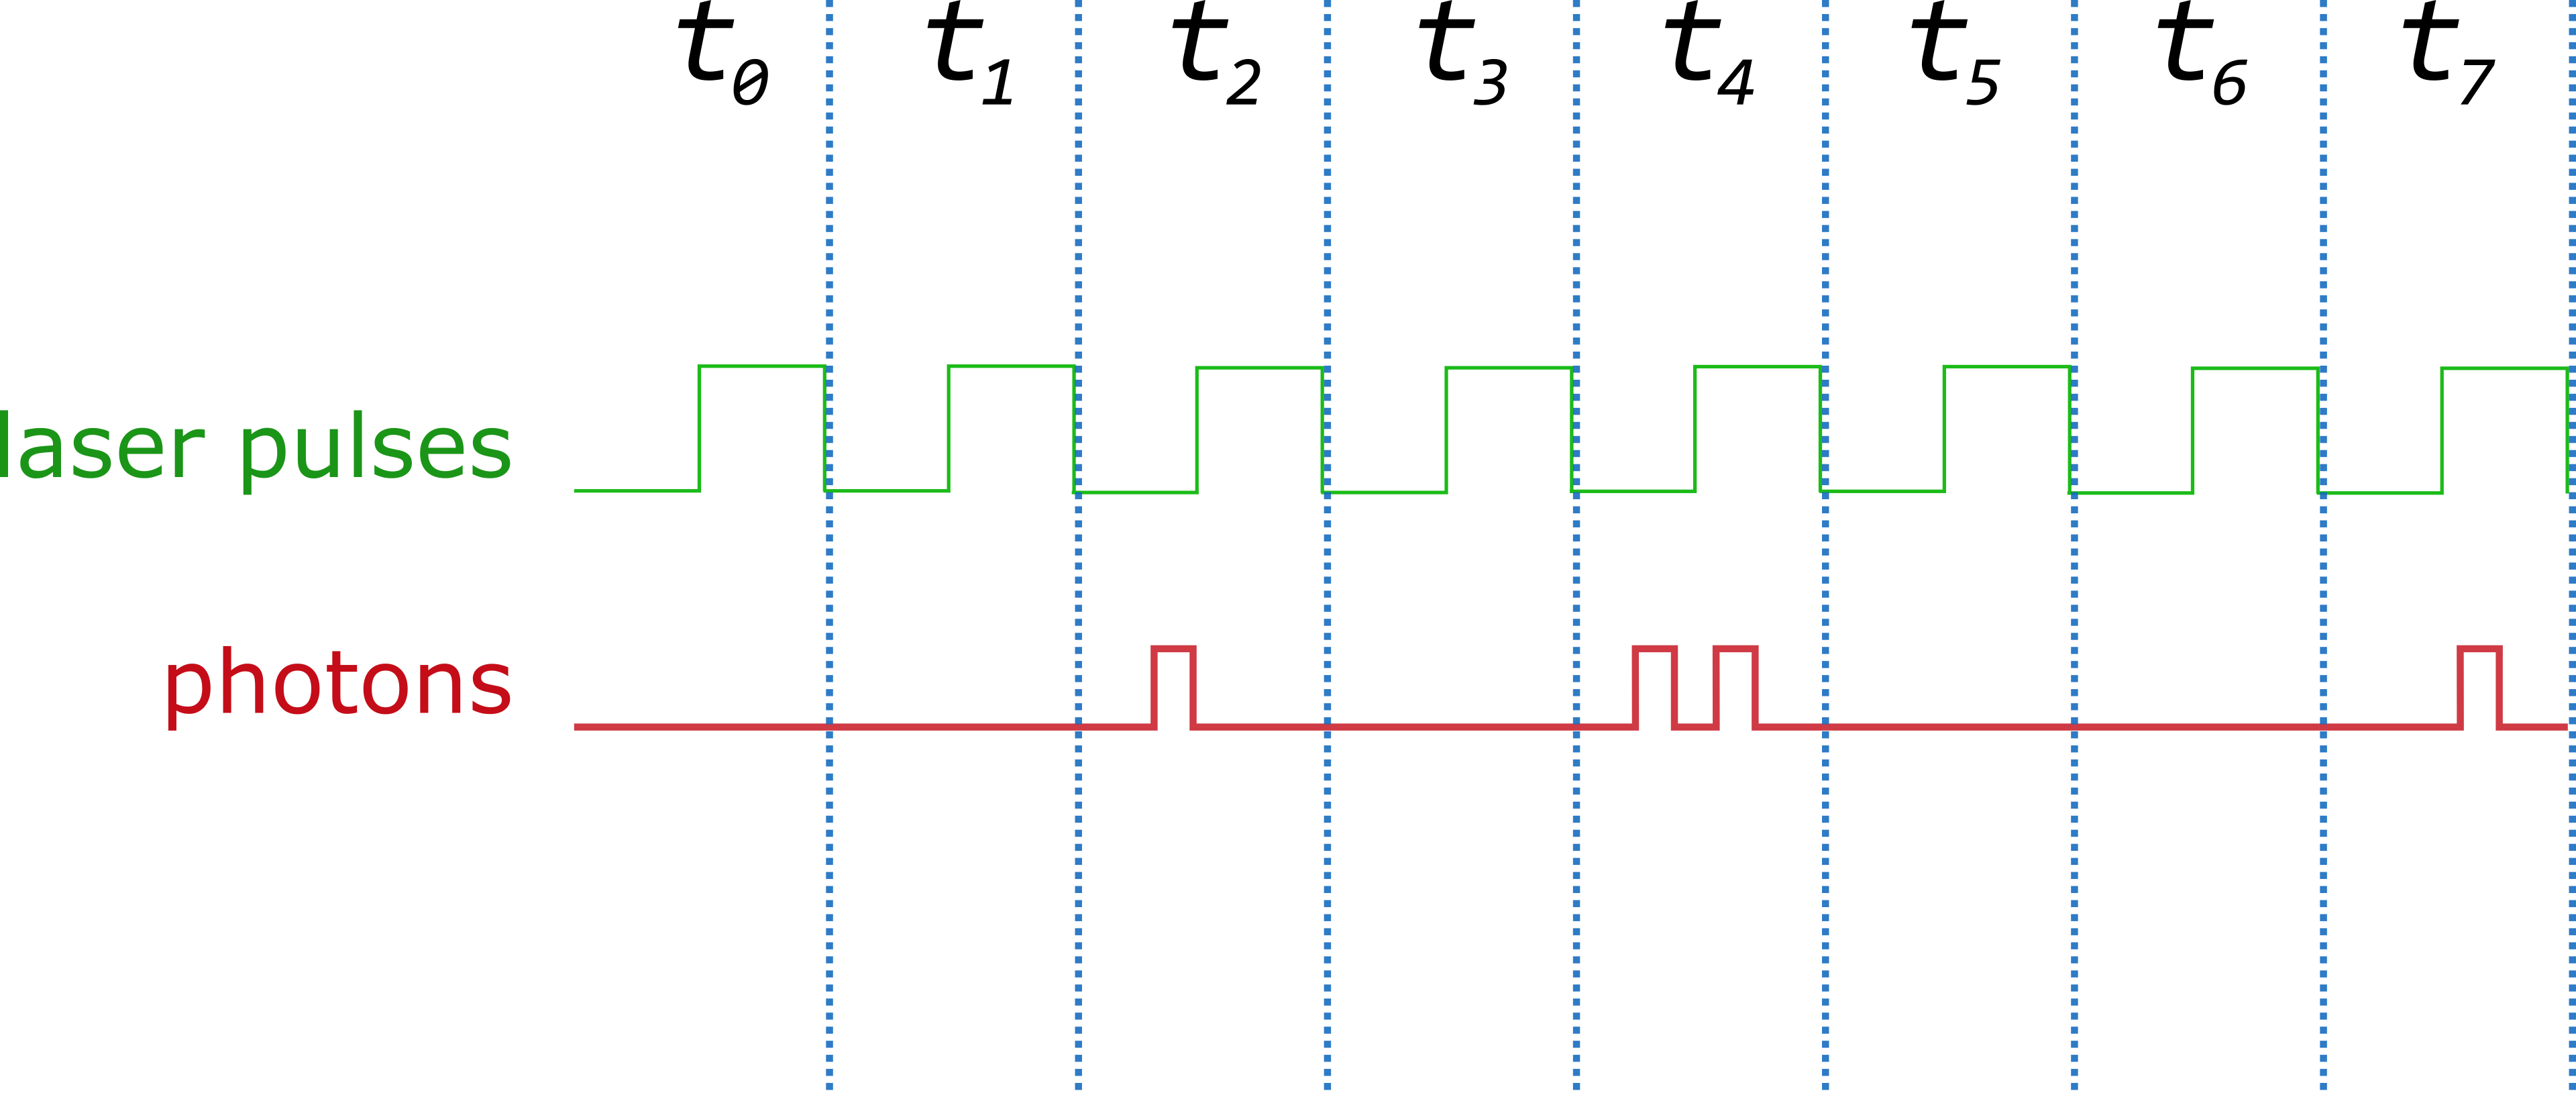
\includegraphics[width=0.7\textwidth]{sample-timing-diagram}
	\caption{Sample FPGA Input Timing Diagram}
	\label{fig:timing}
\end{figure}

\section*{Results}
The simulation software is polished and versatile, able to take input in the form of an image, file, or UNIX pipeline and providing output in both text and graphical form of incident electric field, incident intensity and frequency decomposition, and even an animation in real time. All of these functions will be instrumental in helping the research team design 2D-SPIFI masks, and comparing their performance to a theoretical model. It is also set up in such a way that if the need should arise, the software can double as an analysis tool for real data. The photon counting program on the FPGA works flawlessly with input from a function generator, and will enter testing later this week. The developer will be available for support in the coming months, and there should be a smooth transition with any bugs quickly taken care of.


\section*{Software and Licensing}
Unfortunately, the source code cannot be included here, as the research is still pending publication. At the time of publication, the source will be made available to the community along with its respective documentation.
Once released, the software is provided under the GNU Public License version 3. The simulation is written in the open Python 3.5.2 standard, with a list of free and open source dependencies that will be made available at the same time as the simulation itself. The FPGA code was written using the Quartus software which is the property of Altera$^\textnormal{\small TM}$, along with various pieces of supporting software each of which is subject to its own license. 

\section*{Cost Analysis}
A breakdown of the costs of each of the projects necessary materials is shown in \ref{tbl:cost}.
\begin{table}[h]
\centering
\begin{tabular}{l|r|c|c|r}
\bf{Item} & \bf{Unit Cost} & \bf{Quantity} & \bf{Unit} & \bf{Cost}\\
\hline
Solid State Drive 				& \$95.00 	& 1 & ea 	& \$95.00\\
DEO-Nano FPGA 					& \$86.25 	& 1 & ea 	& \$86.25\\
GPIB-USB Cable					& \$395.00	& 1 & ea 	& \$395.00\\
Mathematica Software License			& \$150.00	& 2 & ea 	& \$300.00\\
\tab$\cdot$Mathematica Subscription Renewal	& \$50.00	& 4 & semester	& \$200.00\\
\hline
Labor 						& \$44.00 	&155& hour	& \$6820.00\\
Overhead	 				& 50\% of Labor	& --& -- 	& \$3410.00\\
\hline
\bf{Total Cost} & & & & \bf{\$11,306.25}
\end{tabular}
\caption{Cost Breakdown for Project Materials\label{tbl:cost}}
\end{table}

The solid state drive is connected to the computer that both manages the FPGA and communicates with the GPIB cable. The GPIB cable was used as a preliminary step in photon counting, using equipment that would perform photon counting with little to no coaxing, but was too archaic to interface with a computer on one of today's hardware standards. Fortunately, the cost of the solid state drive was salvaged as the computer it's connected to now serves as the human interface with the FPGA system. The GPIB-USB cable itself will be repurposed for other projects. Mathematica licenses were required for both a senior member of the research team, and for our team's lead software developer so that he could work with the Mathematica files created by the more senior member. Mathematica has a 1-time payment as well as a regularly-recurring subscription fee, which is proveded on a per-semester basis for students.

\section*{Conclusion}
The ability to reliably simulate 2D SPIFI systems is crucial to the ability
of the other teams working on the broader project to ensure the diffraction
patterns, wheel designs, and optical systems are correct implementations of
the theory, and are operating properly when placed into the system.
Furthermore, the entire point of performing SPIFI microscopy on an object
is to collect the output signal data, making the production of data
collection software imperative to the success of the project. The team
feels that costs of this endeavor are
well worth the advances to science this technology will bring.

Upon the technology's publication, each of these software suites and their
corresponding source code will be made publicly available via a public
source control repository hosted by \href{http://www.gitlab.com}{GitLab}. Though links are provided in the Appendix,
following them will be useless to anyone without access to the
repositories, and will remain so for a little while. It's difficult to say with such things, but the research team expects to be ready to submit an article for peer review by summer's end. To request
access to these repositories, contact the project lead and/or head
software engineer. All links and contact information is available in
Appendix \ref{app:misc}.

\newpage
\section*{Appendix}
\appendix

\section{\label{app:misc}}
\subsection{Contact Information}
\begin{itemize}
\item Project Lead: Dr. Jeff Squire, \href{mailto:jsquier@mines.edu}{jsquier@mines.edu}
\item Team Head Software Engineer: Brennan W. Fieck, \href{mailto:bfieck@mymail.mines.edu}{bfieck@mines.edu}
\end{itemize}
\subsection{Links}
\begin{itemize}
\item \href{https://gitlab.com/PiercingGaze/2DSimulator}{2D SPIFI Mask Simulation Software (unreleased as of the time of this writing)}
\item \href{https://gitlab.com/PiercingGaze/SPIFIDataCollectionSoftware}{Data Collection Suite (unreleased as of the time of this writing)}
\item \href{https://www.researchgate.net/profile/Alyssa_Allende_Motz/publication/281058706_Super-resolved_multimodal_multiphoton_microscopy_with_spatial_frequency-modulated_imaging/links/5790535d08ae64311c0c7dbb.pdf?origin=publication_detail&ev=pub_int_prw_xdl&msrp=c3fj9RD45iTpvk8bRBlzYkN6ndcAYlW9SDWsP0gVb8WzFV5pplCJ3WT6D9fQrP2OT3rGfRWxpWECBz07rTxtH3ZWQ-V2CIIn99KlfPF-otY.9HgCklW2b18-KeSg_Y6vX11zOug1uQ3SSCEpbGXSzk5y_fIuZAdBHJtjk82L1NpfpV2e2Cvcd6QBkqBT24bFzQ.uEqPWNYXdN8Ge_jgkDmRdTlNB8rMwiFPPFdueuZQ9VY6c_KOsp-YvgMVBaNkL6Ldag5ifDVuL2YqcNGnICTcHA}{Original SPIFI Article} - hosted by
\href{https://www.researchgate.net}{Research Gate}
\end{itemize}
\newpage
\begin{thebibliography}{9}

\bibitem{lamport94}
  Dr Jeff Squier. Dr Keith Deluca. et. al.
  \emph{Super-Resolved Multimodal Multiphoton Microscopy with Spatial Frequency-Modulated
Imaging},
  Proceedings of the National Academy of Sciences,
  2015.

\bibitem{boreman}
	Glenn D. Boreman et. al.
	\emph{Use of spatial light modulators in frequency modulation reticle trackers},
	Optical Engineering, November 1990

\bibitem{nih}
	Jeff A. Squier. Michael D. Young. et. al.
	\emph{Eliminating the scattering ambiguity in multifocal, multimodal multiphoton imaging systems},
	J Biophotonicts. 2012 May

\bibitem{micro}
	Michael D. Young.
	"Microfluidic Projection Mask Imaging"
	Colorado School of Mines, Golden. October 20, 2016. Presentation.

\bibitem{Fourier}
	Nicholas George,
	"Fourier Optics," M.S. thesis, Hajim School of Engineering \& Applied Science, University of Rochester, Rochester, NY, 2012

  
\bibitem{talk}
  Futia, Greg. Winters, Dave. Schlup, Philip. Bartels, Dr Randy.
  "Spatial Frequency Modulated Imaging on a Single Element Detector."
  Colorado School of Mines, Golden. May 24, 2011. Presentation.
  

\end{thebibliography}
\end{document}
